\section{Solución Propuesta}

Tomando en cuenta las problematicas mencionadas, se plantea desarrollar una solución que permita al viajero aéreo de la Ciudad de México organizar de manera adecuada su viaje, ofreciendo así una herramienta útil para el ámbito de turismo en México.

La herramienta a desarrollar tendrá la arquitectura que se muestra en la Figura \ref{fig:Arquitectura}. 

\begin{figure}[htbp]
	\centering
		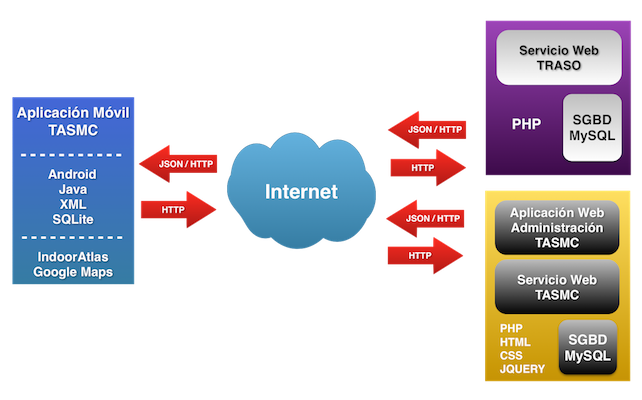
\includegraphics{Figuras/arquitectura.png}
		\rule{35em}{0.5pt}
	\caption[Diagrama de Arquitectura de TASMC]{Diagrama de Arquitectura de TASMC.}
	\label{fig:Arquitectura}
\end{figure}

A continuación se describe cada uno de los componentes que se muestran en la Figura \ref{fig:Arquitectura}:

\begin{itemize}
	\item \textbf{Dispositivo Móvil: }Cuenta con diferentes tecnologías que serán aprovechadas para el desarrollo de la aplicación, por lo tanto, la aplicación móvil será instalada en este dispositivo. Se conectará a la Internet para tener comunicación con el Web Service externo y con el que se desarrollará para este sistema.
	\item \textbf{Web Services: }Se visualizan dos en la Figura \ref{fig:Arquitectura}, uno es el externo que nos brindará la información correspondiente a hoteles y vuelos, y el otro que se desarrollará para brindar la información de los usuarios que utilizan la aplicación. 
	\item \textbf{Servidores: }Observamos dos en la Figura \ref{fig:Arquitectura} que son donde se alojan los Web Services y las Bases de Datos correspondientes, en el servidor TASMC también habrá una aplicación Web.
	\item \textbf{Bases de Datos: }En este módulo encontramos los datos que se proveerán a la aplicación móvil y la aplicación Web.
	\item \textbf{Aplicación Web: }Es una aplicación que servirá para administrar a los usuarios, servicios y objetos de equipaje de la aplicación móvil.
\end{itemize}